\chapter{Discriminative Sentence Alignment}
\label{chap:supervised}

In this chapter we will describe a discriminative models for performing sentence
alignment on comparable document pairs. We use Wikipedia as our first source for
comparable documents, and use a conditional random field \citep{Lafferty01} as
the sentence alignment model. We also apply a discriminative monotonic alignment model to
comparable documents mined from the Web as described by \citet{Uszkoreit10}.

\section{Related Work}
\label{sec:comparable_related}

In addition to aligning parallel texts, there has also been a considerable
amount of work done on finding parallel sentence pairs in comparable corpora. A
comparable corpus is a multilingual collection of documents which may contain
parallel sentences, but is not completely parallel.\adlbr{This seems repetetive, given intro.} 
This broad definition
includes both weakly aligned data such as timestamped multilingual news feeds,
and Wikipedia articles linked at the document level. Depending on the type of
comparable corpus, different methods may be more or less effective for finding
parallel sentences. We will split our review of comparable corpora mining
methods into two categories. In Section \ref{sec:noisy_related}, we will examine
methods used on closely aligned comparable corpora, and in Section
\ref{sec:nonnoisy_related} we will review work on extracting parallel sentences
from less related multilingual documents.

\subsection{Noisy Parallel Corpora}
\label{sec:noisy_related}
The first category of work on comparable corpora mining that we will review is
on noisy parallel data. While even corpora called ``parallel'' contain some
noise, we are refering to corpora which the methods in Section
\ref{sec:parallel_related} would fail on.

Similar to the dynamic programming approaches explored in Section
\ref{sec:parallel_related}, \citet{Zhao02} used a dynamic programming strategy
for aligning parallel sentences in a document pair. They create a probabilistic
model of a comparable document pair $P(S,T,A)$ and choose an alignment to
maximize the probability of the observed source and target documents. To
estimate the probability of two sentences being aligned, they used and IBM-style 
word alignment models (Model 3, specifically) which were estimated on existing
parallel data. \citet{Zhao02} also describes a bootstraping approach where high
confidence sentence alignments are added to the training data for the word
alignment model, and then sentence alignments are recomputed. Much of the work
on noisy parallel/comparable corpora mining used this technique 
\citep{Fung04a,Fung04b,Wu05,Munteanu05}.

\subsection{Finding Parallel Sentences}
Once comparable document pairs have been identified, most comparable corpora
extraction methods will independently judge each sentence pair as parallel or
non-parallel. Since there is often a very large amount of document pairs and
thus potential sentence pairs, filters are used to prune out sentence pairs that
are highly unlikely to be parallel. For example, \citet{Munteanu05} used a
sentence length filter to remove sentence pairs where one sentence was more than
twice as long as the other. In addition, they used a word overlap filter based
on the bilingual dictionary used to find candidate document pairs.

Given a filtered set of sentence pairs, more expensive methods of scoring
sentence pairs can be used. \citet{Munteanu05} use a binary MaxEnt
classifier to ultimately determine whether or not a sentence pair is parallel.
The classifier is trained on parallel data and makes used of features which are
mostly based on word alignments. Others
\cite{Fung04a,Fung04b,Tillmann09a,Tillmann09b} use a single score for sentence
pairs based on either a word alignment model or bag-of-words similarity after
projection through a bilingual lexicon, and tune a threshold on held out data.

\section{Wikipedia as a Comparable Corpus}
\label{sec:wiki}
Wikipedia \citep{wikipedia} is an online collaborative encyclopedia available in
a wide variety of languages.  While the English Wikipedia is the largest, with
over 3 million articles, there are 24 language editions with at least 100,000
articles.

Articles on the same topic in different languages are also connected via
``interwiki'' links, which are annotated by users.  This is an extremely
valuable resource when extracting parallel sentences, as the document alignment
is already provided.  
Table \ref{table:interwiki} shows how
many of these ``interwiki'' links are present between the English Wikipedia and the
16 largest non-English Wikipedias.

\begin{table*}
\small
\begin{center}
\begin{tabular}{|c|c|c|c|c|c|c|c|}
\hline
French & German & Polish & Italian & Dutch & Portuguese & Spanish & Japanese \\
496K & 488K & 384K & 380K & 357K & 323K & 311K & 252K\\
\hline
Russian & Swedish & Finnish & Chinese & Norwegian & Volap\"{u}k & Catalan & Czech \\
232K & 197K & 146K & 142K & 141K & 106K & 103K & 87K\\
\hline
\end{tabular}
\end{center}
\caption{Number of aligned bilingual articles in Wikipedia by language (paired with English).}
\label{table:interwiki}
\end{table*}

Wikipedia's markup contains other useful indicators for parallel sentence
extraction.  The many hyperlinks found in articles have previously been used as
a valuable source of information.  \citep{Adafre06} use matching
hyperlinks to identify similar sentences.  Two links match if the articles they
refer to are connected by an ``interwiki'' link.
Also, images in Wikipedia are often stored in a central source across
different languages; this allows identification of captions which may be
parallel.  Finally, there are other minor forms
of markup which may be useful for finding similar content across languages, such
as lists and section headings.  In Section \ref{sec:features}, we will explain
how features are derived from this markup.

\section{Models for Parallel Sentence Extraction}
\label{sec:models} In this section, we will focus on methods for
extracting parallel sentences from aligned, comparable documents.
The related problem of automatic document alignment in news and
web corpora has been explored by a number of researchers,
including
\citet{Resnik03}, \citet{Munteanu05},
\citet{Tillmann09a}, and \citet{Tillmann09b}.
Since our corpus already contains document alignments, we sidestep
this problem, and will not discuss further details of this issue.
That said, we believe that our methods will be effective in
corpora without document alignments when combined with one of the
aforementioned algorithms.


\subsection{Binary Classifiers and Rankers}
Much of the previous work involves building a binary classifier for sentence
pairs to determine whether or not they are parallel
\citep{Munteanu05,Tillmann09a}.
The training data usually comes from a standard parallel corpus.  There is a
substantial class imbalance ($O(n)$ positive examples, and $O(n^2)$
negative examples), and various heuristics are used to mitigate this problem.
\citet{Munteanu05} filter out negative
examples with high length difference or low word overlap (based on a bilingual
dictionary).

We propose an alternative approach: we learn a ranking model, which, for each sentence in the {\em
source} document, selects either a sentence in the {\em target} document that it is
parallel to, or ``null''.
This formulation of the problem avoids the class imbalance issue of the binary classifier.

In both the binary classifier approach and the ranking approach, we use a Maximum Entropy
classifier, following \citet{Munteanu05}.

\subsection{Sequence Models}
In Wikipedia article pairs, it is common for parallel sentences to
occur in clusters.  A global sentence alignment model is
able to capture this phenomenon. For both parallel and comparable
corpora, global sentence alignments have been used, though the
alignments were monotonic
\citep{Gale93,Moore02,Zhao02}.
Our model is a first order linear chain conditional random field
(CRF) \citep{Lafferty01}. The set of source and
target sentences are observed. For each {\em source} sentence, we
have a hidden variable indicating the corresponding {\em target}
sentence to which it is aligned (or null). The model is similar to the
discriminative CRF-based word alignment model of
\citep{Blunsom06}.

\subsection{Features}
\label{sec:features}
Our features can be grouped into four categories.

\subsubsection{Features derived from word alignments}
%kristina-edit-1

We use a feature set inspired by \citep{Munteanu05}, who defined
features primarily based on IBM Model 1 alignments
\citep{Brown93}.  We also use HMM word alignments
\citep{Vogel96} in both directions ({\em source} to {\em target} and
{\em target} to {\em source}), and extract the following features based on these
four alignments:\footnote{These are all derived from the one best alignment, and
normalized by sentence length.}

\begin{enumerate}
\item Log probability of the alignment
\item Number of aligned/unaligned words
\item Longest aligned/unaligned sequence of words
\item Number of words with fertility 1, 2, and 3+
\end{enumerate}

We also define two more features which are independent of word alignment
models.  One is a sentence length feature taken from \citep{Moore02}, which
models the length ratio between the {\em source} and {\em target} sentences with
a Poisson distribution.  The other feature is the difference in relative
document position of the two sentences, capturing the idea that the aligned
articles have a similar topic progression.

The above features are all defined on sentence pairs, and are included in the
binary classifier and ranking model.
\subsubsection{Distortion features} In the sequence model, we use additional distortion
features, which only look at the difference between the position
of the previous and current aligned sentences.  One set of
features bins these distances; another looks at the
absolute difference between the expected position (one after the
previous aligned sentence) and the actual position.

\subsubsection{Features derived from Wikipedia markup}

Three features are derived from Wikipedia's
markup. The first is the number of matching links in the sentence
pair. The links are weighted by their inverse frequency in the
document, so a link that appears often does not contribute much to
this feature's value.  The image feature fires whenever two
sentences are captions of the same image, and the list feature
fires when two sentences are both items in a list.  These last two
indicator features fire with a negative value when the feature
matches on one sentence and not the other.

None of the above features fire on a null alignment, in either the
ranker or CRF.  There is also a bias feature for these two models, which
fires on all non-null alignments.

\subsubsection{Word-level induced lexicon features}
In order to address sparsity issues in our seed parallel corpora, we introduce a
bilingual lexicon model which learns word translation probabilities from the
linked Wikipedia articles. The details of this model and the features derived
from it can be found in \citep{Smith10}.

\section{Experiments}
\label{sec:exp}

\subsection{Data}
We annotated twenty Wikipedia article pairs for three language pairs: Spanish-English,
Bulgarian-English, and German-English.
Each sentence in the {\em source} language was annotated with
possible parallel sentences in the {\em target} language (the target language was
English in all experiments).  The pairs were annotated with a quality level:
{\bf 1} if the sentences contained some parallel fragments, {\bf 2} if the sentences
were mostly parallel with some missing words, and {\bf 3} if the sentences appeared to be direct
translations.  In all experiments, sentence pairs with quality {\bf 2} or {\bf 3} were
taken as positive examples. 

\begin{table*}[ht]
\tiny
\begin{center}
\begin{tabular}{|c||c|c|c||c|c|c||c|c|c|}
\hline
Language Pair     & \multicolumn{3}{|c||}{Binary Classifier} & \multicolumn{3}{|c||}{Ranker} & \multicolumn{3}{|c|}{CRF} \\
\hline
                  & Avg Prec & R@90 & R@80
                  & Avg Prec & R@90 & R@80
                  & Avg Prec & R@90 & R@80 \\
\hline
English-Bulgarian & 75.7  & 33.9  & 56.2    & 76.3  & 38.8  & 57.0    & {\bf 80.6}  & {\bf 52.9}  & {\bf 59.5} \\
English-Spanish   & 90.4  & 81.3  & 87.6    & 93.4  & 81.0  & 84.5    & {\bf 94.7}  & {\bf 87.6}  & {\bf 90.2} \\
English-German    & 61.8  &  9.4  & 27.5    & 66.4  & 25.7  & 42.4    & {\bf 78.9}  & {\bf 52.2}  & {\bf 54.7} \\
\hline
\end{tabular}
\end{center}
\caption{Average precision, recall at 90\% precision, and recall at 80\%
precision for each model in all three language pairs.  In these experiments, the
Wikipedia features and lexicon features are omitted.}
\label{table:modelcompare}
\end{table*}

\begin{table*}[ht]
\small
\begin{center}
\begin{tabular}{|c||c|c|c||c|c|c|}
\hline
Setting           & \multicolumn{3}{|c||}{Ranker} & \multicolumn{3}{|c|}{CRF} \\
\hline
                  & Avg Prec & R@90 & R@80
                  & Avg Prec & R@90 & R@80\\
\hline
English-Bulgarian & & & & & & \\
\hline
One Direction          & 76.3  & 38.8  & 57.0    & 80.6  & 52.9  & 59.5 \\
Intersected            & 78.2  & 47.9  & 60.3    & 79.9  & 38.8  & 57.0 \\
Intersected +Wiki      & 80.8  & 39.7  & 68.6    & 82.1  & 53.7  & 62.8 \\
Intersected +Wiki +Lex & 89.3  & 64.4  & 79.3    & {\bf 90.9}  & {\bf 72.0}  & {\bf 81.8} \\
\hline
English-Spanish & & & & & & \\
\hline
One Direction          & 93.4  & 81.0  & 84.5    & 94.7  & 87.6  & 90.2 \\
Intersected            & 94.3  & 82.4  & 89.0    & 95.4  & 88.5  & 91.8 \\
Intersected +Wiki      & 94.5  & 82.4  & 89.0    & 95.6  & 89.2  & 92.7 \\
Intersected +Wiki +Lex & 95.8  & 87.4  & 91.1    & {\bf 96.4}  & {\bf 90.4}  & {\bf 93.7} \\
\hline
English-German & & & & & & \\
\hline
One Direction          & 66.4  & 25.7  & 42.4    & 78.9  & 52.2  & 54.7 \\
Intersected            & 71.9  & 36.2  & 43.8    & 80.9  & 54.0  & 67.0 \\
Intersected +Wiki      & 74.0  & 38.8  & 45.3    & 82.4  & 56.9  & {\bf 71.0} \\
Intersected +Wiki +Lex & 78.7  & 46.4  & 59.1    & {\bf 83.9}  & {\bf 58.7}  & 68.8 \\
\hline
\end{tabular}
\end{center}
\caption{Average precision, recall at 90\% precision, and recall at 80\%
precision for the Ranker and CRF in all three language pairs.  ``+Wiki''
indicates that Wikipedia features were used, and ``+Lex'' means the lexicon
features were used.}
\label{table:featurecompare}
\end{table*}

For our seed parallel data, we used the Europarl corpus
\citep{Koehn05} for Spanish and German and the
JRC-Aquis corpus for Bulgarian, plus the article titles for
parallel Wikipedia documents, and translations available from
Wiktionary entries.\footnote{Wiktionary is an online collaborative
dictionary, similar to Wikipedia.} %kristina-edit

\subsection{Intrinsic Evaluation}
Using 5-fold cross-validation on the 20 document pairs for each
language condition, we compared the binary classifier, ranker, and
CRF models for parallel sentence extraction. To tune for 
precision/recall, we used minimum Bayes risk decoding.  We define
the loss $L(\tau,\mu)$ of picking target sentence $\tau$ when the
correct target sentence is $\mu$ as $0$ if $\tau=\mu$, $\lambda$ if
$\tau = \textsc{null}$ and $\mu\ne\textsc{null}$, and $1$ otherwise.
By modifying the null loss $\lambda$, the precision/recall
trade-off can be adjusted.  For the CRF model, we used posterior
decoding to make the minimum risk decision rule tractable. As a
summary measure of the performance of the models at different
levels of recall we use average precision as defined in
\citep{Ido06}. We also report recall at precision of 90 and
80 percent. %kristina-edit 
 Table \ref{table:modelcompare} compares the
different models in all three language pairs.

In our next set of experiments, we looked at the effects of the Wikipedia
specific features.  Since the ranker and CRF are asymmetric models,
we also experimented with running the models in both directions and combining
their outputs by intersection.  These results are shown in Table \ref{table:featurecompare}.

Identifying the agreement between two asymmetric models is a commonly
exploited trick elsewhere in machine translation. It is mostly effective
here as well, improving all cases except for the Bulgarian-English CRF where
the regression is slight. More successful are the Wikipedia features, which
provide an auxiliary signal of potential parallelism.

The gains from adding the lexicon-based features can be dramatic
as in the case of Bulgarian (the CRF model average precision
increased by nearly 9 points). The lower gains on Spanish and
German may be due in part to the lack of language-specific
training data. These results are very promising and
motivate further exploration. We also note that this
is perhaps the first successful practical application of an
automatically induced word translation lexicon.

\subsection{SMT Evaluation}

We also present results in the context of a full machine translation system
to evaluate the potential utility of this data.  A standard
phrasal SMT system \citep{Koehn03} serves as our testbed, using
a conventional set of models: phrasal models of source given target and
target given source; lexical weighting models in both directions, language
model, word count, phrase count, distortion penalty, and a lexicalized
reordering model.  Given that the extracted Wikipedia data takes the
standard form of parallel sentences, it would be easy to exploit this same
data in a number of systems.

\begin{table*}[ht]
\tiny
\begin{center}
\begin{tabular}{|rr||r|r||r|r||r|r|}
\hline
      &                & German        & English       & Spanish       & English      & Bulgarian    & English   \\
\hline
      & sentences     & 924,416       & 924,416       & 957,884       & 957,884      & 413,514      & 413,514   \\
\textbf{Medium} \
      & types     & 351,411       & 320,597       & 272,139       & 247,465      & 115,756      & 69,002    \\
      & tokens    & 11,556,988    & 11,751,138    & 18,229,085    & 17,184,070   & 10,207,565   & 10,422,415\\
\hline
      & sentences      & 6,693,568     & 6,693,568     & 7,727,256     & 7,727,256    & 1,459,900    & 1,459,900 \\
\textbf{Large} \
      &      types     & 1,050,832     & 875,041       & 1,024,793     & 952,161      & 239,076      & 137,227   \\
      &      tokens    & 100,456,622   & 96,035,475    & 155,626,085   & 137,559,844  & 29,741,936   & 29,889,020\\
\hline
      & sentences      & 1,694,595     & 1,694,595     & 1,914,978     & 1,914,978    & 146,465      & 146,465   \\
\textbf{Wiki}  \
      &      types     & 578,371       & 525,617       & 569,518       & 498,765      & 107,690      & 74,389    \\
      &      tokens    & 21,991,377    & 23,290,765    & 29,859,332    & 28,270,223   & 1,455,458    & 1,516,231 \\
\hline
\end{tabular}
\end{center}
\caption{Statistics of the training data size in all three language pairs.}
\label{table:mtTrainStats}
\end{table*}

\begin{table*}[ht]
\small
\begin{center}
\begin{tabular}{|rr||r|r||r|r||r|r|}
\hline
      &                & German        & English       & Spanish       & English      & Bulgarian     & English   \\
\hline
\textbf{Dev A} \
      & sentences      & 2,000         & 2,000         & 2,000         & 2,000        & 2,000         & 2,000     \\
      & tokens    & 16,367        & 16,903        & 24,571        & 21,493       & 39,796        & 40,503    \\
\hline
\textbf{Test A}\
      & sentences      & 5,000         & 5,000         & 5,000         & 5,000        & 2,473         & 2,473     \\
      & tokens    & 42,766        & 43,929        & 68,036        & 60,380       & 52,370        & 52,343    \\
\hline
\textbf{Wikitest}\
      & sentences    & 500           & 500           & 500           & 500          & 516           & 516       \\
      & tokens    & 8,235         & 9,176         & 10,446        & 9,701        & 7,300         & 7,701     \\
\hline
\end{tabular}
\end{center}
\caption{Statistics of the test data sets.}
\label{table:mtTestStats}
\end{table*}

For each language pair we explored two training conditions.  The
``Medium'' data
condition used easily downloadable corpora: Europarl for German-English and
Spanish-English, and JRC/Acquis for Bulgarian-English.  Additionally we
included titles of all linked Wikipedia articles as parallel sentences in
the medium data condition.  The ``Large'' data condition includes all the
medium
data, and also includes using a broad range of available sources such as
data scraped from the web~\citep{Resnik03}, data from the United
Nations, phrase books, software documentation, and more.

In each condition, we explored the impact of including additional
parallel sentences automatically extracted from Wikipedia in the
system training data. For German-English and Spanish-English, we
extracted data with the null loss adjusted to
achieve an estimated precision of 95 percent, and for
English-Bulgarian a precision of 90 percent. %kristina-edit-1
Table~\ref{table:mtTrainStats} summarizes the characteristics of
these data sets.  We were pleasantly surprised at the amount of
parallel sentences extracted from such a varied comparable corpus.
Apparently the average Wikipedia article contains at least a
handful of parallel sentences, suggesting this is a very fertile
ground for training MT systems.

The extracted Wikipedia data is likely to make the greatest impact on broad
domain test sets -- indeed, initial experimentation showed little BLEU gain
on in-domain test sets such as Europarl, where out-of-domain training data
is unlikely to provide appropriate phrasal translations.  Therefore, we
experimented with two broad domain test sets.

First, Bing Translator provided a sample of translation
requests along with translations in German-English and
Spanish-English -- this constituted our standard development and
test set for those language pairs.  Unfortunately no such tagged
set was available in Bulgarian-English, so we held out a portion
of the large system's training data to use for development and
test. In each language pair, the test set was split into a
development portion (``Dev A'') used for minimum error rate
training~\citep{OchMert03} and a test set (``Test A'') used
for final evaluation.

\begin{table*}[ht!]
\small
\begin{center}
\begin{tabular}{|lr||l||l|l|}
\hline
Language pair     & Training data     & Dev A             & Test A            & Wikitest     \\
\hline
Spanish-English   & Medium            & 32.6              & 30.5              & 33.0         \\
                  & Medium+Wiki       & 36.7 (+4.1)       & 33.8 (+3.3)       & 39.1 (+6.1)  \\
                  & Large             & 39.2              & \textbf{37.4}     & 38.9         \\
                  & Large+Wiki        &\textbf{39.5} (+0.3)&37.3 (-0.1)       & \textbf{41.1} (+2.2)  \\
\hline
German-English    & Medium            & 28.7              & 26.6              & 13.0         \\
                  & Medium+Wiki       & 31.5 (+2.8)       & 29.6 (+3.0)       & 18.2 (+5.2)  \\
                  & Large             & \textbf{35.0}     & 33.7              & 17.1         \\
                  & Large+Wiki        & 34.8 (-0.2)       &\textbf{33.9} (+0.2)&\textbf{20.2} (+3.1)  \\
\hline
Bulgarian-English & Medium            & 36.9              & 26.0              & 27.8         \\
                  & Medium+Wiki       & 37.9 (+1.0)       & 27.6 (+1.6)       & 37.9 (+10.1) \\
                  & Large             &\textbf{51.7}      &\textbf{49.6}      & 36.0         \\
                  & Large+Wiki        &\textbf{51.7}(+0.0)& 49.4 (-0.2)       &\textbf{39.5}(+3.5)  \\
\hline
\end{tabular}
\end{center}
\caption{BLEU scores of MT systems under various training and test
conditions.  The final BLEU score from minimum error rate training is in the
first column; two additional columns are BLEU scores on held-out test sets.
For training data conditions including the extracted Wikipedia sentences,
the parenthesized values indicate the absolute BLEU difference against the
corresponding system without Wikipedia extracts.}
\label{table:mtTestResults}
\end{table*}

Second, we created new test sets in each of the three language
pairs by sampling parallel sentences from held out Wikipedia
articles.  To ensure that this test data was clean, we manually
filtered the sentence pairs that were not truly parallel and
edited them as necessary to improve adequacy.  We called
this ``Wikitest''. Characteristics of
these test sets are summarized in Table~\ref{table:mtTestStats}.

We evaluated the resulting systems using
BLEU-4~\citep{Papineni02}; the results are presented in
Table~\ref{table:mtTestResults}.  First we note that the extracted
Wikipedia data are very helpful in medium data conditions,
significantly improving translation performance in all conditions.
Furthermore we found that the extracted Wikipedia sentences
substantially improved translation quality on held-out Wikipedia
articles. In every case, training on medium data plus Wikipedia
extracts led to equal or better translation quality than the large
system alone. Furthermore, adding the Wikipedia data to the large
data condition still made substantial improvements.

\section{Comparable documents from the Web}

Multilingual websites have often been used as a source of parallel data
\citep{Resnik03,Huang05,Shi06}. Most approaches for finding potential parallel
documents rely on metadata rather than the content of the websites. 
This metadata may include links which appear to point to alternate versions of the same
page in another language, the URLs of the websites, or their HTML structure.
Another approach for finding multilingual websites is given by
\citet{Uszkoreit10}, who translate all non-English web pages into English using
their MT system and then use monolingual document similarity measures to find
comparable document pairs. \citet{Uszkoreit10} also describe a sentence
alignment model which is applied to the comparable document pairs. In this work,
we will instead use a discriminative, monotonic alignment model to align these document
pairs. As this requires labeled sentence alignment data for both training and
evaluation, we also describe an annotation tool for monotonic alignments which 
allows $m:n$ sentence matchings.

\subsection{Data collection}

\subsubsection{Annotation Tool}

\begin{figure}
\begin{center}
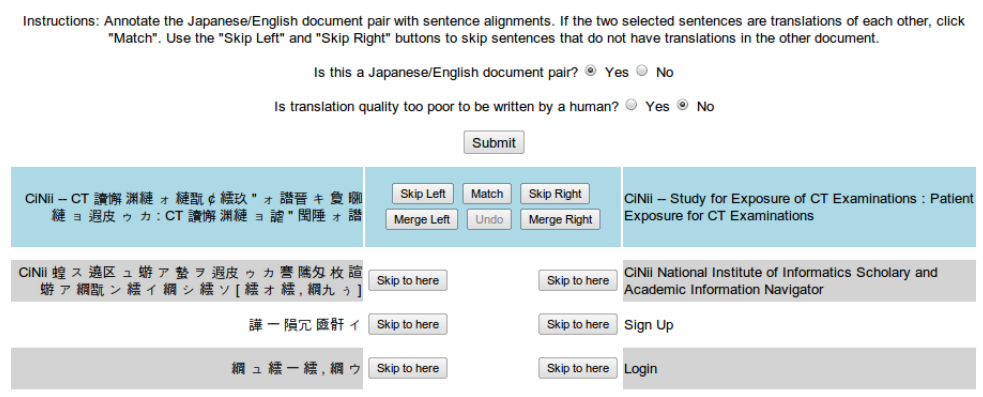
\includegraphics[scale=0.5]{images/google_annotate.png}
\caption{The annotation interface for sentence alignment.
\NoteJS{Take or adapt the figure from the Google slides.}
}
\label{fig:google_annotate}
\end{center}
\end{figure}

We obtain a set of Japanese-English document pairs using the method described by
\citet{Uszkoreit10}. From this set, we randomly selected roughly 1000 document
pairs to be annotated. The annotators were presented with the interface shown in
Figure \ref{fig:google_annotate}. For each document pair we asked if
the two documents are in the correct language pair, and if one of the documents
appeared to be machine translated. If the language pair was correct and the
documents appeared to be translated by a human, then the annotators aligned the
sentences in the document.

The annotation tool is closely related to the monotonic alignment model in how
it operates. The user is asked whether or not the first sentences in each
document are parallel. If they are, the user selects ``Match'', the sentences
are aligned, and the user is then prompted about the next two sentences. If the
sentence pair presented to the annotator is not parallel, they will select
either ``Skip Left'' or ``Skip Right'', which advance the current sentence in
the document on the left or right. These three operations correspond to the
operations used in the monotonic alignment model, and the annotator's sequence
of operations can be directly used as training data.

The tool also allows the annotator to specify arbitrary $n:m$ sentence
alignments throught the ``Merge Left'' and ``Merge Right'' buttons. The merge
actions append the immediately following sentences to the currently selected
sentences, which can then be aligned.

\subsubsection{Data Collection Results}

Since the data we have annotated using this tool is taken from the HTML source
of webpages, and converted to plain text and segmented into sentences
automatically, the ``Merge'' buttons are often used to correct errors in
sentence segmentation. This results in a few large $n:m$ alignments, though most
alignments are still $1:1$. Table \ref{table:merge_stats} breaks down the
alignments that the annotators have provided.

\begin{table*}[ht!]
\begin{center}
\begin{tabular}{|l||l|l|l|l|l|}
\hline
Alignment Type & 1:1 & 2:1 & 1:2 & 2:2 & Other\\
\hline
Percentage & 95.8\% & 1.70\% & 1.28\% & 0.159\% & 1.12\%\\
\hline
\end{tabular}
\end{center}
\caption{Statistics on the types of $n:m$ alignments found in the annotated
data.}
\label{table:merge_stats}
\end{table*}

\subsection{Monotonic alignment model}

\begin{figure}
\begin{center}
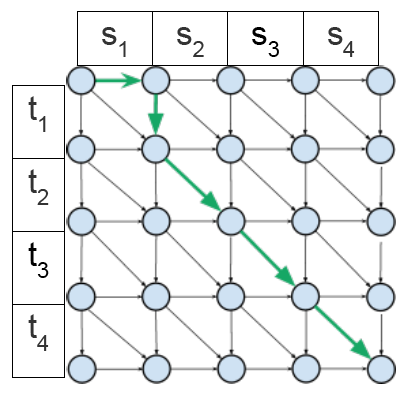
\includegraphics[scale=0.5]{images/google_model.png}
\caption{The discriminative model for monotonic sentence alignment. The
highlighted path represents a possible alignment between the two documents.}
\label{fig:mono_disc}
\end{center}
\end{figure}

Our sentence alignment model is a discriminatively trained monotonic alignment
model. An illustration of this model is given in Figure \ref{fig:mono_disc}.
Formally, we represent the model as a weighted finite-state automata (WFSA) with features
that fire on each arc as described in \citet{Eisner02}. Specifically, in this
work we use a weighted finite-state transducer (WFST) to describe our alignment
model. A WFST includes a set of states
$\mathbb{Q}$, source and target alphabets $\Sigma_S$ and $\Sigma_T$,
transition function $\delta : \mathbb{Q} \times \Sigma_S \times \Sigma_T
\longrightarrow \mathbb{Q} \times W$,
and start and end states $\mathbb{S}$ and $\mathbb{F}$.

\begin{align*}
\mathbb{Q} &=& \{q_{i,j} \mid 0 \leq i \leq |\vec{S}|, 0 \leq j \leq |\vec{T}|\}\\
\Sigma_S &=& \{\epsilon\} \cup \{S_i \mid 0 \leq i < |\vec{S}|\}\\
\Sigma_T &=& \{\epsilon\} \cup \{T_j \mid 0 \leq j < |\vec{T}|\}\\
\delta(q_{i, j}) &=& \{(q_{i+1, j}, (S_i, \epsilon), \vec{f}(S_i, \epsilon)\cdot\vec{w}),\\
& & (q_{i, j+1}, (\epsilon, T_j), \vec{f}(\epsilon, T_j)\cdot\vec{w}),\\
& & (q_{i+1,j+1}, (S_i, T_j), \vec{f}(S_i, T_j)\cdot\vec{w})\}\\
\mathbb{S} &=& q_{0,0}\\
\mathbb{F} &=& q_{|\vec{S}|, |\vec{T}|}
\end{align*}

\NoteJS{The transition function still needs some work, and I need to mention
semirings. A section on notation should help with this.}

The FSM representing the set of possible alignments for a document pair 
$(\vec{S}, \vec{T})$ has $(|\vec{S}|+1)\cdot(|\vec{T}|+1)$ states. These states
correspond to positions in the source and target documents. Each state has at
most three transitions, which either skip the current source sentence, skip the
current target sentence, or align the current source and target sentences. Note
that these operations directly match the actions used by the annotators to
generate the labeled alignments, so they may be directly used as an observed
path through the WFSA. This automata only contains $1:1$ alignments, though
$n:m$ alignments could be added to this machine through additional arcs on each
state.

The weights on each of the arcs $a$ come from the dot product of the features which
fire on that arc and the weight vector $\vec{w}$. 
The total weight of a path $\pi = a_0,a_1,\dots,a_n$ is the dot product of all
features firing on each arc and the weight vector. Using this property we can
now define a probability distribution over paths through this WFST:

\begin{align*}
p(\pi|\vec{S}, \vec{T}) &=& \frac{\sum_{a \in \pi}
\exp \vec{f}(a)\cdot\vec{w}}{\sum_{\pi'}\sum_{a \in \pi'}\exp \vec{f}(a)\cdot\vec{w}}
\end{align*}

The denominator is the sum of the weights of all paths through the WFST.
We train our model to maximize the probability of the observed training data:

\begin{align*}
\argmax{\vec{w}} \sum_{(\pi,\vec{S},\vec{T})} p(\pi|\vec{S},\vec{T})
\end{align*}

The gradient of this objective can be computed using standard finite-state
algorithms \citep{Eisner02}.

\subsubsection{Features}
\label{sec:mono_feats}
We chose to use a simple set of features which are mostly based on
bag-of-words similarity measures. First, we have bias features which fire on all
``matching'' and ``mismatching'' arcs (arcs which emit $(S_i, T_j)$ are matching
arcs, and the mismatching arcs emit either $(\epsilon, T_j)$ or $(S_i,
\epsilon)$). For the matching arcs, we project the source sentence through a
weighted bilingual dictionary and compute cosine similarity with the target
sentence (and the same is done in reverse).\NoteJS{I don't have the exact set of
features used in the experiments from my Google slides.}

We also experimented with a set of first-order features, which look at the
previous arc taken in the WFST. This is made possible by splitting each state
$q_{i,j}$ into $q_{i,j,+}$ and $q_{i,j,-}$. ``Match'' transitions lead to
$q_{i,j,+}$ while ``mismatch'' transitions lead to $q_{i,j,-}$. Since the states
are now recording the last operation, the arcs leaving these states have
features which fire on two matches in a row, for example. The intuition behind
adding these features is that matches often follow other matches, and a similar
trend is present for mismatches.

\subsection{Results}

We compare our discriminatively trained model against a hand-tuned monotonic
alignment model. Our results are shown in Table \ref{table:google_results}.

\begin{table*}
\begin{center}
\begin{tabular}{|l||l|l|l|}
\hline
Model & Precision & Recall & F1\\
\hline
\hline
Baseline & 63.9\% & 95.0\% & 76.4\%\\
\hline
Discriminative Aligner & {\bf 66.0\%} & 94.4\% & {\bf 77.7}\%\\
\hline
+First Order Features & 65.1\% & {\bf 95.2\%} & 77.3\%\\
\hline
\end{tabular}
\caption{Precision, recall and F1 score measured on a held out set of aligned
Japanese-English document pairs.}
\label{table:google_results}
\end{center}
\end{table*}
